\documentclass[11pt]{article}
\usepackage[parfill]{parskip}
\usepackage{graphicx}
\usepackage{wrapfig}
\usepackage{subcaption}
\usepackage[top=1in, bottom=1in, left=1in, right=1in]{geometry}
\bibliographystyle{plain}
\usepackage{amsmath}
\usepackage{amsfonts}
\usepackage{hyperref}
\usepackage{listings}
\usepackage{xcolor}
%%%%%%%%%%%%%%%%%%%%%%%%%%%%%%%%%%%%%%%%%%%%%%%%%%%%%%%%%%%%%%%
\usepackage{fancyhdr}
\pagestyle{fancy}
%%% Please add the author's last names
\lhead{Galois TA2 AMIDOL}
\rhead{ASKE Milestone 5 Report}
%%% Please use \cfoot{} to remove page numbers
\cfoot{ }
\renewcommand{\headrulewidth}{0pt}
\renewcommand{\footrulewidth}{0pt}
%%%%%%%%%%%%%%%%%%%%%%%%%%%%%%%%%%%%%%%%%%%%%%%%%%%%%%%%%%%%%%&
\usepackage{titlesec}
\titlespacing{\section}{0pt}{\parskip}{-.5\parskip}
\titlespacing{\subsection}{0pt}{\parskip}{- .5\parskip}
\titlespacing{\subsubsection}{0pt}{\parskip}{- .5\parskip}
\newcommand{\closeup}{\setlength{\itemsep}{-4pt}}

\colorlet{punct}{red!60!black}
\definecolor{background}{HTML}{EEEEEE}
\definecolor{delim}{RGB}{20,105,176}
\colorlet{numb}{magenta!60!black}

\lstdefinelanguage{json}{
    basicstyle=\normalfont\ttfamily,
    numbers=left,
    numberstyle=\scriptsize,
    stepnumber=1,
    numbersep=8pt,
    showstringspaces=false,
    breaklines=true,
    frame=lines,
    backgroundcolor=\color{background},
    literate=
     *{0}{{{\color{numb}0}}}{1}
      {1}{{{\color{numb}1}}}{1}
      {2}{{{\color{numb}2}}}{1}
      {3}{{{\color{numb}3}}}{1}
      {4}{{{\color{numb}4}}}{1}
      {5}{{{\color{numb}5}}}{1}
      {6}{{{\color{numb}6}}}{1}
      {7}{{{\color{numb}7}}}{1}
      {8}{{{\color{numb}8}}}{1}
      {9}{{{\color{numb}9}}}{1}
      {:}{{{\color{punct}{:}}}}{1}
      {,}{{{\color{punct}{,}}}}{1}
      {\{}{{{\color{delim}{\{}}}}{1}
      {\}}{{{\color{delim}{\}}}}}{1}
      {[}{{{\color{delim}{[}}}}{1}
      {]}{{{\color{delim}{]}}}}{1},
}

\newcommand{\amidol}{\textsc{AMIDOL}}

\def\signed #1{{\leavevmode\unskip\nobreak\hfil\penalty50\hskip2em
  \hbox{}\nobreak\hfil(#1)%
  \parfillskip=0pt \finalhyphendemerits=0 \endgraf}}

\newsavebox\mybox
\newenvironment{aquote}[1]
  {\savebox\mybox{#1}\begin{quote}}
  {\signed{\usebox\mybox}\end{quote}}

\date{\vspace{-5ex}}
% Use this to get rid of the date

\usepackage{authblk}
\author[1]{Eric Davis}
\author[1]{Alec Theriault}
\author[1]{Ryan Wright}
\affil[1]{Galois, Inc}

%\setcounter{page}{0}



\title{April ASKE Milestone 5 Report for \amidol{}}

\begin{document}
\maketitle
\vspace{10pt}

\section{Introduction}

The initial prototype of \amidol{} has been implemented as a proof of
concept, and platform for developing the theories, algorithms, core
architectures, domain specific languages, and intermediate
representations from our original proposal.  This prototype represents
an advancement on the state-of-the-art for creating, solving, and
analyzing complex models from scientific, physical, social, and hybrid
domains.  \amidol{} aims to reduce the overhead associated with the
model life cycle and to enable domain experts and scientists to more
easily build, maintain, and reason over models in robust and highly
performable ways, and to respond rapidly to emerging crises in an
agile and impactful way.  The initial prototype achieves these goals
by implementing several Visual Domain Specific Ontological Languages
(VDSOLs), a novel intermediate representation whose representation is
based on existing formalisms such as Markov models
\cite{howard2012dynamic}, Generalized Stochastic Petri-nets with
inhibitor arcs \cite{chiola1993generalized}, and stochastic activity
networks \cite{movaghar1985performability,sanders2000stochastic}.

\amidol{}'s VDSOLs are designed to lower the barrier for entry
associated with formal modeling languages, and the long term costs
associated with model maintenance.  VDSOLs allow the expression of
rich mathematical concepts using visual diagrams for systems and
processes.  Because \amidol{} uses a universal representation for this
intermediate form, models defined with \amidol{} can be easily ported
to off the shelf solution techniques which have already been vetted by
the community, and optimized for high performance computing.
\amidol{} models are also amenable to sharing, as their common
intermediate representation means they can translated to different
languages and representations, and composed with other models, even
those generated with other formalisms.

The Phase 1 Prototype for \amidol{} shows a proof of concept of the
core capabilities required to achieve this full vision in Phase 2, and
has helped to identify the necessary next steps in realizing a the
full framework as part of the ASKE program.  We include in our
prototype three VDSOLs to show flexibility, and two backend targets
already in use by the community.  The backend targets utilized by our
prototype further help demonstrate our core capabilities by
translating models in \amidol{}'s IR into PySCeS based models, and
systems of differential equations, showing \amidol{}'s ability to
utilize the IR to translate into other formalisms easily,
automatically, and performably.

\section{Initial Prototypes}

The initial prototype for \amidol{} is implemented as a front-end user
interface, using HTML, CSS, and Javascript, communicating with the
Scala back-end using JSON over HTTP.  This client/server approach
leverages standard browser technologies for rapid development of rich
interactions tailored for the specific needs of scientific
modeling. It also decouples the concerns of visual presentation and
manipulation from the underlying representations of model semantics
and helps to hide the details from domain experts reducing their
cognitive load when designing models.

Our initial prototype employs a rich visual editor allowing users to
select a palette to work in, to save and load VDSOL diagrams, undo and
redo operations, to customize parameters exposed by nouns and verbs,
to define reward variables on a diagram, and to call multiple backend
solver targets to solve those reward variables. Currently, the user
interface implements a visual editor for directed graphs having
labeled vertices and edges, which represent the nouns and verbs of a
VDSOL.

Each VDSOL is implemented as a palette which is defined externally and
provides a set of nouns and verbs specific to the domain, along with a
translation protocol from the VDSOL into the IR.

\begin{figure}
  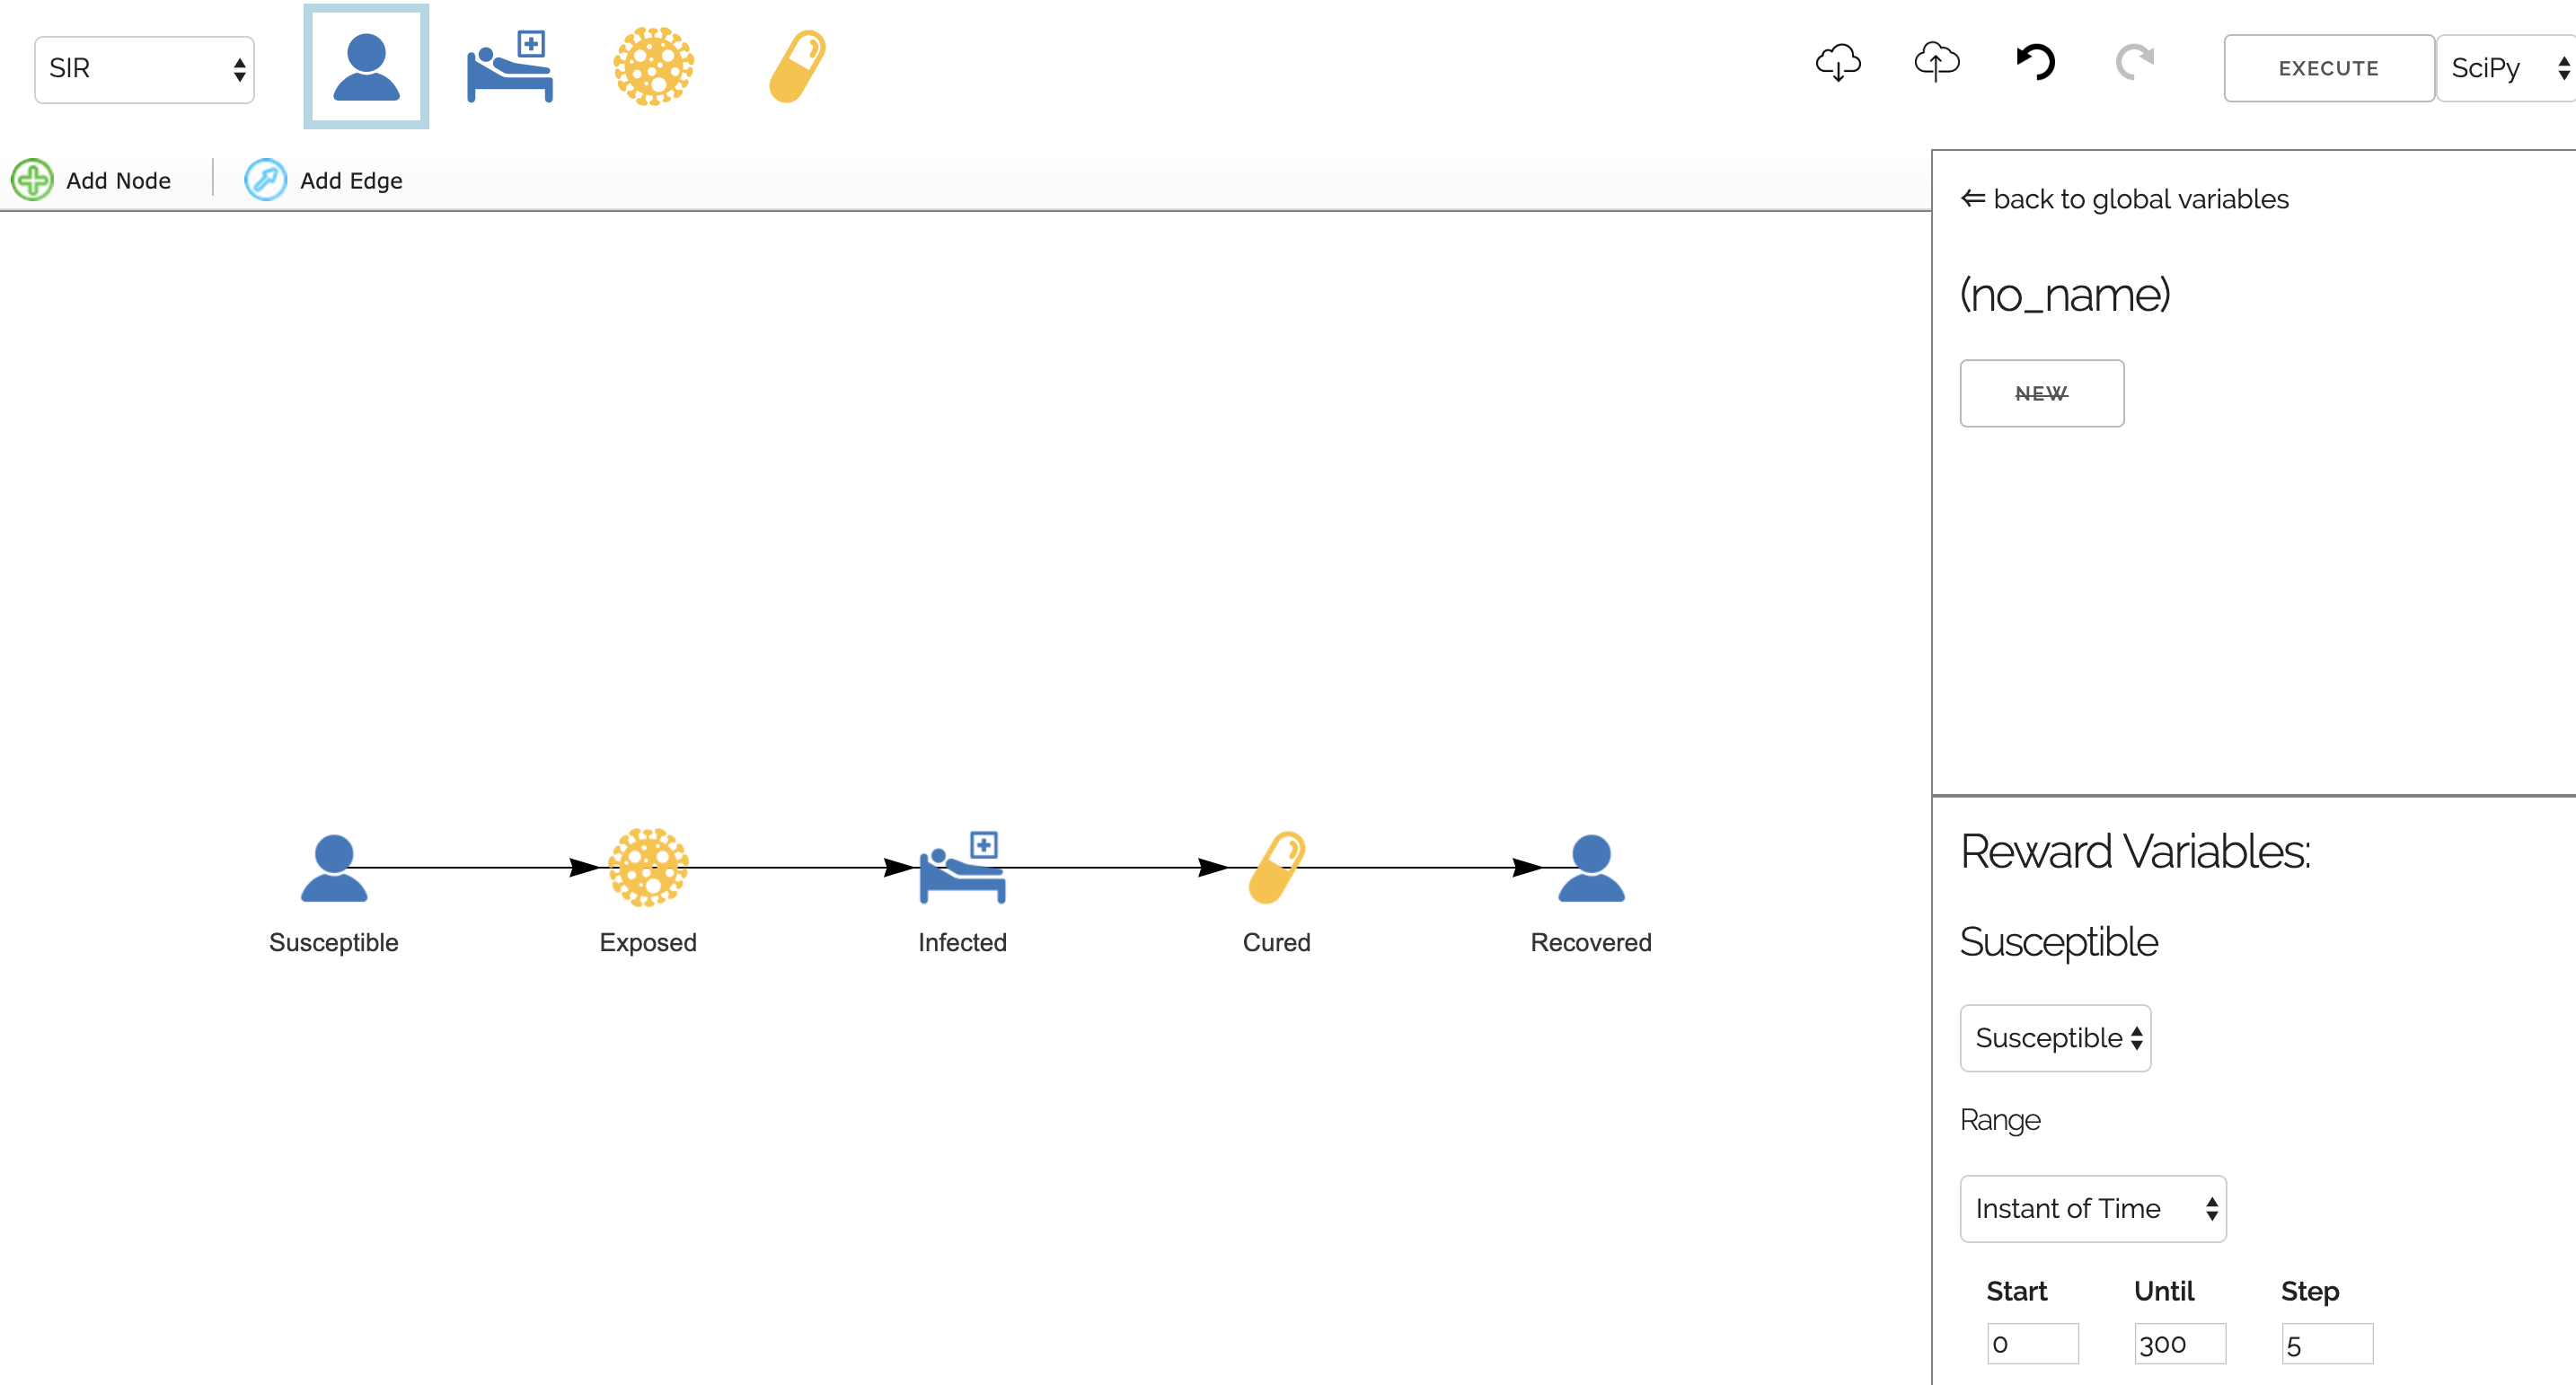
\includegraphics[width=\textwidth]{figs/SIR.png}
  \caption{\amidol{} prototype with SIR Model}
\label{Fig:SIR-Proto}
\end{figure}

Figure \ref{Fig:SIR-Proto} shows the a standard SIR infection model
implemented using the SIR palette.  This model can be solved either
through translation into ODEs, or to the PySCeS model formalism, but
it can also be used an example of the power of VDSOLs and palette
extension.  The palettes defined for \amidol{} can be modified, and
even extended, easily by adding new nouns and verbs.  This allows for
the long term curation of models by domain experts, who can easily
extend their earlier work as new processes and interactions are
discovered.

\begin{figure}
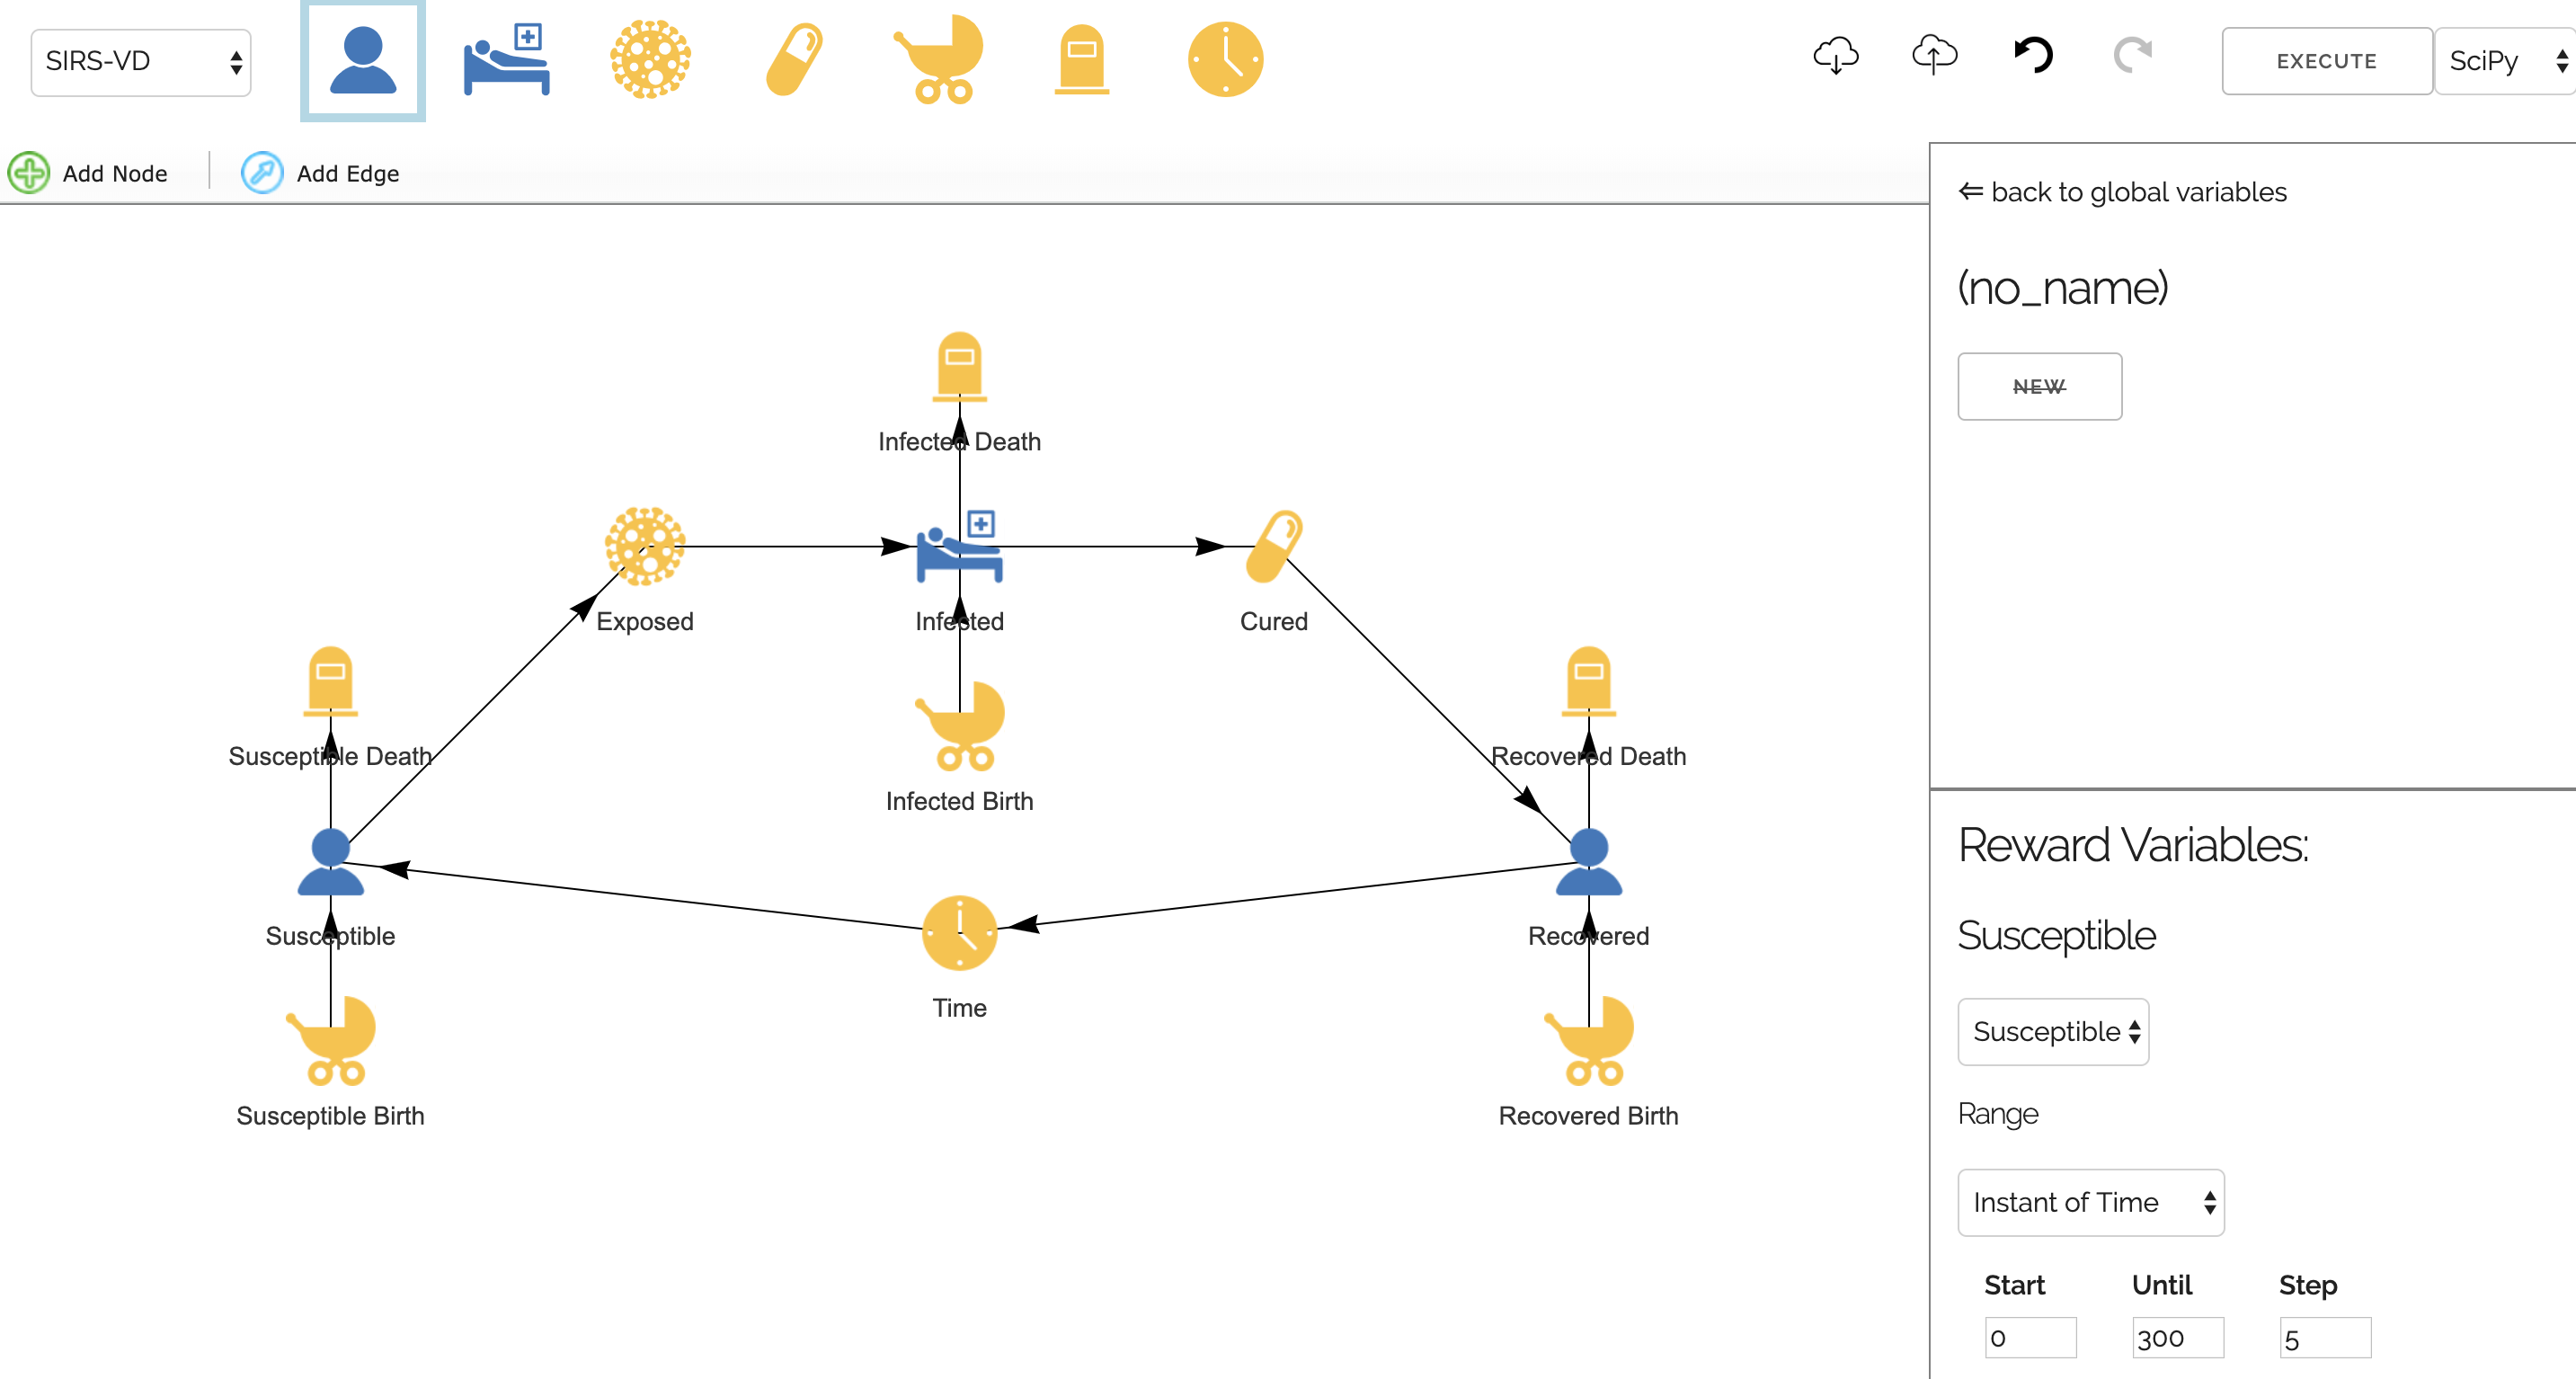
\includegraphics[width=\textwidth]{figs/SIR-VD.png}
\caption{\amidol{} prototype with SIR Model with Vital Dynamics}
\label{Fig:SIR-VD-Proto}
\end{figure}

Figure \ref{Fig:SIR-VD-Proto} shows an example of such an extension,
adding verbs for birth and death from a population.  Our hope is this
capability improves the longevity of models defined in \amidol{},
ensuring fewer models die on the shelf from neglect and bitrot, or
simply are not reused due to changes in solver technology, or
advancements in algorithms.

As an example of a wholly different palette for a VDSOL, and to
demonstrate the capability of our Phase 1 prototype to handle models
in different domains, we have also implemented a domain model for the
Lotka-Volterra model of predator-prey relationships, shown in Figure \ref{Fig:LV-Proto}
\cite{freedman1980deterministic,brauer2012mathematical,hoppensteadt2006predator}.
Frequently used to describe the basic dynamics of biological systems
with two species interactions, the Lotka-Volterra model assumes a
single predator, and single prey species.  While a simple model, this
system is an example of a Kolmogorov model which is used as the
underlying framework for modeling other dynamic systems, such as
competing species in a niche, the impact of disease on a species, and
mutualistic relationships.  It is provided in our initial prototype
primarily as another model for which it is easy to validate and
generate expectations, and to demonstrate the capacity of our
prototype to work in multiple domains.

\begin{eqnarray}
  \frac{dx}{dt} &=& \alpha x - \beta x y\\
  \frac{dy}{dt} &=& \delta x y - \gamma y
\end{eqnarray}

\begin{figure}
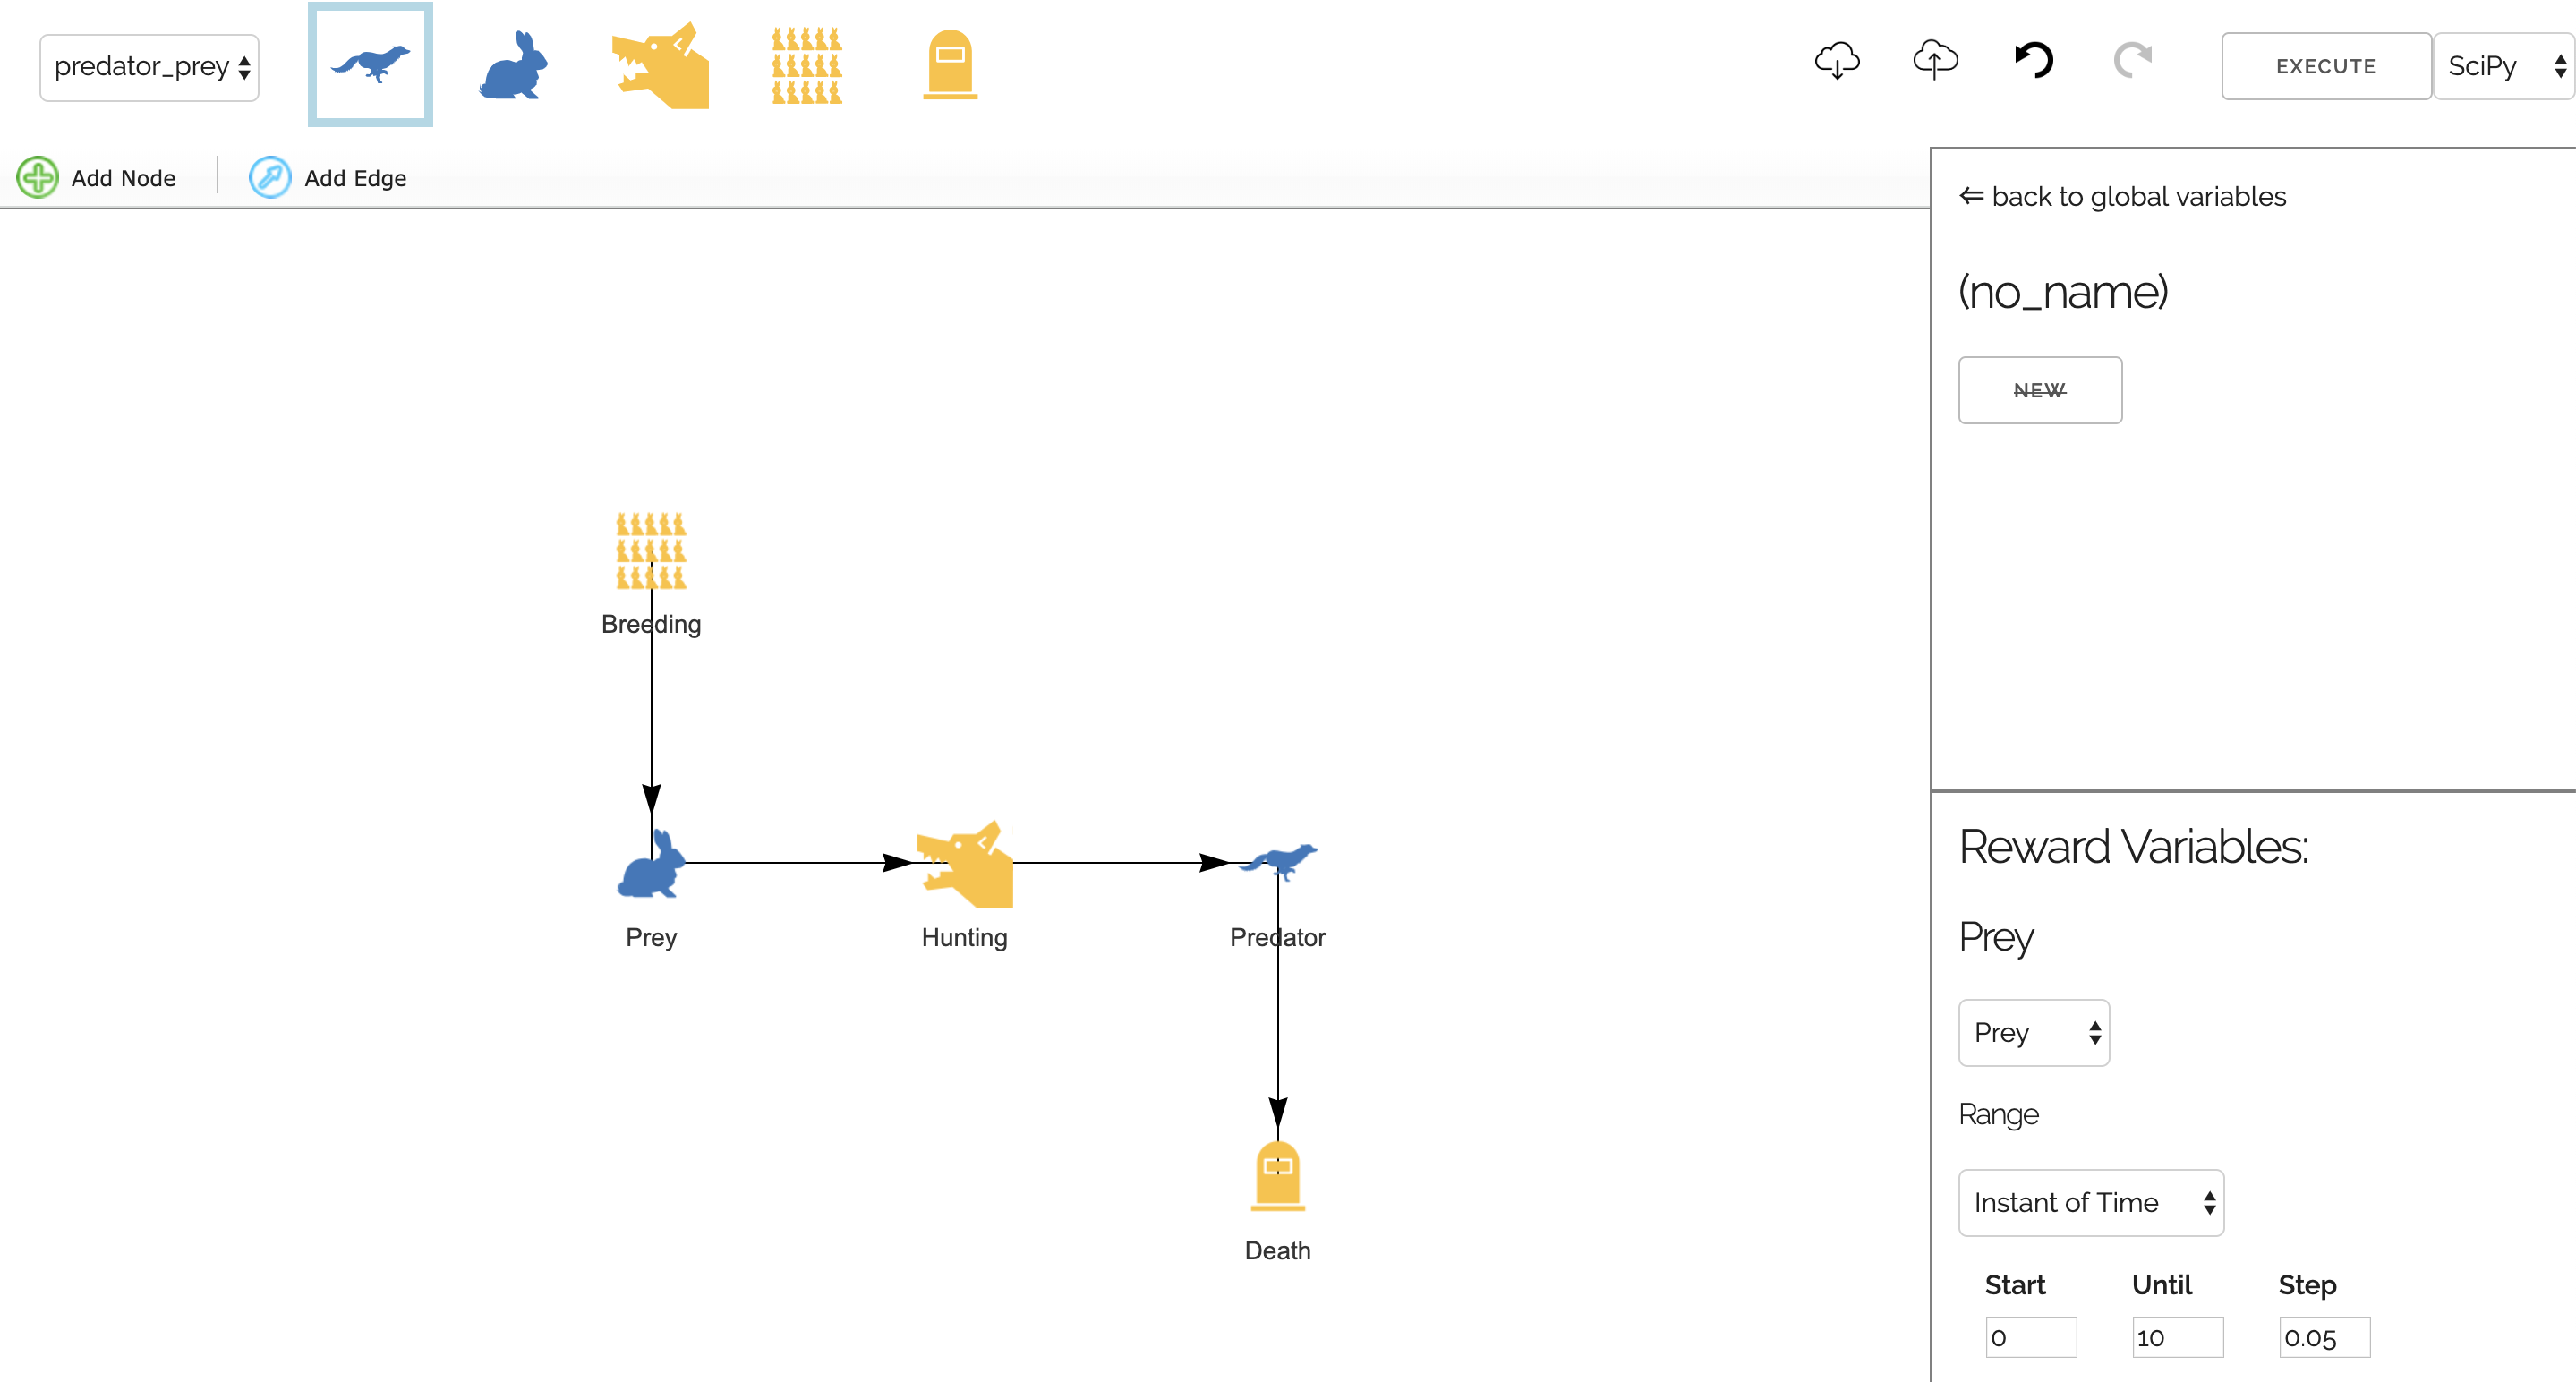
\includegraphics[width=\textwidth]{figs/Pred-Prey.png}
\caption{\amidol{} prototype with Lotka-Volterra Model}
\label{Fig:LV-Proto}
\end{figure}

\section{Road Map for the Future}

The Phase 1 prototype for \amidol{} has proved the core technologies
and functionality required for success in this project are feasible,
achievable, and provide the necessary functionality to support our
vision for Phase 2.  Phase 2 will work on extending this base
functionality and building on top of our current architecture.  During
Phase 2 we will work with more complex models, including full models
of H3N2 and H5N1 which include multiple geographic compartments.
Phase 1 has also helped us to understand key challenges and
capabilities which need to be developed in Phase 2 in order to make
\amidol{} a more fully functional system for complex modeling.  We
divide these challenges into three core areas: \textbf{Model
  Creation}, \textbf{Model Analysis}, and \textbf{Long-term Goals}.
The next sections will address these challenges, as well as the sub
challenges identified below.

\begin{itemize}
\item Model Creation
  \begin{itemize}
  \item VDSOL Expressivity
  \item Composability of Models
  \item Model Transformation and Optimization
  \end{itemize}
\item Model Analysis
  \begin{itemize}
  \item Reward Definition
  \item New Solver Targets
  \item Results Database
  \end{itemize}
\item Long-term Goals
  \begin{itemize}
  \item Model Synthesis
  \end{itemize}
\end{itemize}

\section{Challenges to Model Creation}

\subsection{VDSOL Expressivity}

One major improvement our Phase 1 work has highlighted is the need to
extend our VDSOLs to include support for multigraphs and hypergraphs
\cite{balakrishnan2012textbook,berge1984hypergraphs}.  While current
VDSOL palettes implemented by our prototype allow for some expressive
models in their chosen domains, we have identified several additional
capabilities regarding edge assignment, and node state-variable
exposure, which warrant additional UI/UX innovation.  Take, for
example, the following model of viral replication
\cite{srivastava2002stochastic,haseltine2002approximate}:

\begin{eqnarray}
  \mathrm{LTR} \overset{k_{\mathrm{basal}}}{\rightarrow} \mathrm{LTR} + \mathrm{nRNA}\\
  \mathrm{nRNA} \overset{k_{\mathrm{export}}}{\rightarrow} \mathrm{cRNA}\\
  \mathrm{cRNA} \overset{k1_{\mathrm{translate}}}{\rightarrow} \mathrm{GFP} + \mathrm{cRNA}\\
  \mathrm{cRNA} \overset{k2_{\mathrm{translate}}}{\rightarrow} \mathrm{Tat} + \mathrm{cRNA}\\
  \mathrm{Tat}
  \overset{k_{\mathrm{bind}}/k_{\mathrm{unbind}}}{\leftrightarrow} \mathrm{pTEFb}_d\\
  \mathrm{LTR} + \mathrm{pTEFb}_d \overset{k_{\mathrm{acetyl}}/k_{\mathrm{deacetly}}}{\leftrightarrow} \mathrm{pTEFb}_a\\
  \mathrm{pTEFb}_a  \overset{k_{\mathrm{transact}}}{\rightarrow} \mathrm{LTR} + \mathrm{nRNA} + \mathrm{Tat}\\
  \mathrm{GFP} \overset{d_{\mathrm{GFP}}}{\rightarrow} \emptyset\\
  \mathrm{Tat} \overset{d_{\mathrm{Tat}}}{\rightarrow} \emptyset\\
  \mathrm{cRNA} \overset{d_{\mathrm{CYT}}}{\rightarrow} \emptyset\\
  \mathrm{nRNA} \overset{d_{\mathrm{NUC}}}{\rightarrow} \emptyset\\
\end{eqnarray}

This fairly simple model has some rather complex dynamics, and
requires a VDSOL capable of implementing stoichiometry.  In particular,
our current palettes do not support the catalyzing reactions, such as
that represented by the first equation.  LTR is not consumed in this
reaction, yet its concentration is vital to the state dependent rate
represented by $k_{\mathrm{basal}}$.  In order to support this, our
palette must support linking of inputs and outputs in a verb, to
ensure easy definition of preserved reactants, and specification of
partial and total orders on inputs and outputs when inputs and outputs
cannot be treated as a single composed state variable.

The primary challenge here isn't theoretical, such systems can easily
be created with modest extensions of \amidol{}'s Phase 1
capabilities.  They are primary around the user experience, and
human-machine teaming aspects of VDSOL representation.  We intend to
explore this design space, and to include such UI/UX considerations in
our extension to formal palette definitions.

\subsection{Composibility of Models}

In addition to increased expressivity from VDSOL extensions, \amidol{}
is being designed to support the composition of individual models in
Phase 2 to enable model reuse, compositional methods for solution, and
to allow domain scientists to experiment by
swapping out components of a model which may represent complex
hypotheses about individual elements.  Composition is an essential
element of the long-term model development lifestyle for \amidol{},
and a key feature for collaborative science and knowledge extraction.

Composition is currently partially implemented in the Phase 1
prototype as the method for building an IR model from nouns and verbs
in a given VDSOL.  For Phase 2, \amidol{} will be extended, providing
an editor in the UI to define custom compositions of atomic models via
state-sharing.  Variables which are shared between two composed models
have the same marking, or value, and are effected by events in both
models.

Composition will allow more rich model development, and model
development as a modular and collaborative task, similar to working on
separate objects or packages in code development.  VDSOL
representations of atomic models can be synchronized across members of
a team, and edited individually, then composed in a similar way to
object code with external references in software engineering.

\subsection{Model Transformation and Optimization}

The last major target for improving model creation in \amidol{} is the
implementation of a full set of primitive transformations on the IR
representations of a model.  \amidol{}'s architecture is designed in
an analogous way to LLVM \cite{lattner2004llvm,lattner2008llvm} and
similarly is designed for multistage optimization and transformation
on the intermediate representation \cite{lattner2002llvm}.
\amidol{}'s IR is, in a sense, like a byte code language for models
allowing the backend to perform transformations on models defined in
this IR, acting on models via well structured transformations as shown
in Figure \ref{Fig:AMIDOLBackend}.  While VDSOLs provide benefits by
being diverse and adapted to various domains, the \amidol{} IR
provides benefits by being universal, allowing transformations to be
leveraged across domains in a consistent and verifiable manner.

Currently \amidol{} implements composition operators as the basic
operation needed to combine nouns, verbs, and reward variables into an
executable model, and the translation of multiple VDSOLs into the
IR. In Phase 2 we will extend \amidol{} to account for all of this 
proposed functionality.

\begin{figure}
  \begin{eqnarray}
    \mathrm{translate}(\mathrm{VDSOL}_A) & \rightarrow & \mathrm{IR}_A\\
    \mathrm{compose}(\mathrm{IR}_A, \mathrm{IR}_B) & \rightarrow & \mathrm{IR}_C\\
    \mathrm{translate}(\mathrm{IR}_A) & \rightarrow & \mathrm{target}_A\\
    \mathrm{optimize}(\mathrm{IR}_A)) & \rightarrow & \mathrm{IR}_B\\
    \mathrm{equivalence}(\mathrm{IR}_A, \mathrm{IR}_B) & \rightarrow & \mathrm{True} \vee \mathrm{False}
  \end{eqnarray}
  \caption{}
  \label{Fig:AMIDOLBackend}
\end{figure}

\section{Challenges for Analysis}

In addition to challenges in model definition and development, Phase 2
of \amidol{} will address challenges for model analysis,
interrogation, and querying.  The primary ways this will be
accomplished will include richer reward definition, new solver targets
to support more robust analysis, and the implementation of a results database.

\subsection{Reward Definition}

The current Phase 1 prototype of \amidol{} implements only rate
rewards for instant of time.  During Phase 2 we will implement impulse
rewards, and enable interval of time and steady state reward variables
of both rate and impulse types. Steady state reward variables will
make heavy use of our ability to perform transformations on the IR, as
they represent an often wholly different solution target.

In addition to supporting a wider variety of atomic reward variables,
Phase 2 will focus on extending reward variables to allow for composed
rewards as expressions defined over atomic and composed reward
variables. While atomic reward variables form the
basis for model evaluation, \amidol{} will support expressions defined
over reward variables using basic arithmetic operations allowing
reward variables to be composed via normal mathematical expressions.

\subsection{New Solver Targets}

Phase 1 supports a limited number of solvers, which mostly focus on
interpreting models as systems of differential equations.  During
Phase 2 will support additional transformations to allow for discrete
event solution as a target, along with numerical solution via
successive matrix multiplication for models with finite state spaces.

Because different solution techniques are required by more complex
reward variables, a key part of the backend for Phase 2 will be
constraint identification and satisfaction, which will solve multiple
reward variables with potentially different solvers and techniques for
the same model, the results of which will be fed into a results
database for later synthesis and composed reward solution.  This
backend architecture helps to ensure the performability of models
designed in \amidol{}, and flexibility of solution technique helping
researchers avoid the pitfall of being bound to a single target using
hand coded models, which may or may not be performable.

\subsection{Results Database}

The final major component to our model analysis goals for Phase 2 is
the creation of a results database to support explainability goals by
tying the results of solving reward variables back to the primitives
present in the VDSOL, storing intermediate results, allowing for the
construction of complex composed rewards across models (allowing for
model comparison), and allowing for the definition of ``data-driven''
models which can ingest traces, and real data from external sources as
realizations of reward variables for model fitting, and testing.

Tying the results of model solution to elements in the VDSOL is a key
goal of \amidol{}. Reward variable in models are currently defined on
model primitives such as
state variables and events, which are elements of our IR and not a
given VDSOL.  This is not ideal for our goals and desired outcomes
which focus on expert interaction with the VDSOL while hiding details
of the underlying model.  During Phase 2 we will extend this
definition to provide equivalent higher level constructs for rate and
impulse rewards which are instead defined more naturally over nouns
and verbs.  We propose doing so by defining reward measurement points in an
extension of our VDSO, indicating what a measure on a noun or a
verb will return.  This is a natural extension of our current palette
definitions for VDSOLs which define input and output predicate
connections. These new capabilities will allow users to naturally
define reward variables and will allow us to infer information on
\textbf{structural types} of nouns and verbs, determine equivalences,
and capture knowledge from domain experts when they tell us they
believe nouns in two different models represent the same abstract
quantity.

The results of these reward variables will be stored in a database of
prior results, and interacted with in a Design of Experiments
interface.  This Design of Experiments interface will allow a user to perform
complex analyses on models, comparisons with past executions,
comparisons with other models, and comparisons with empirical data
using composed rewards.  This interface and database will support the
complex queries and prognostics required by the original BAA.  This interface
will borrow from concepts of Plackett-Burman
designs, and factorial designs using individual reward variables and
parameterizations defined over a given model as atomic components of
expressions.  Computations for given atomic components will be stored
in the results database to avoid unneeded reevaluation, and to allow
future experiments to build on past results, and be directly compared
and contrasted.

The Design of Experiments interface will also allow users to load data
from external sources, and associate this data with expectations for
state variables in the model.  In our early tests we have achieved
this by using data from the CDC's Fluview \cite{cdc2019fluview} data
sets as series of instant-of-time observations.  \amidol{}'s interface
will allow users to use regression to estimate the conditional
expectation of dependent variables, given independent variables with
fixed values from the data, allowing prediction, parameter estimation,
and later risk assessment for a given regression through analysis of
the distribution of possible realizations for state variables in a
given model.

Our new interface will also allow direct comparison through user
identification of reward variables, or expressions on reward
variables, in two models which represent comparable properties or
processes allowing the exploration of alternatives, conditional
forecasting, counterfactual analysis, and comparative impact.
Different strategies, configurations, or possible outcomes can be
explored through examining different ways to parameterize a given
model, or even differences in models with structural changes.
Debugging experiments will be enabled through the connections to the
VDSOL ontology.  For instance, the interface will allow users to see
the direct dependence of reward variables to noun's and verbs in the
original ontology, better enabling researchers to understand the
knowledge-based semantic dependencies normally hidden by traditional
modeling techniques.

Because we will allow for factorial and Plackett-Burman experiment
design users will be able to
automatically perform one-factor-at-a-time
\cite{bailis2005mortality,murphy2004quantification} sensitivity and
uncertainty estimates.  The initial prototype will also feature
screening sampling-based methods \cite{morris1991factorial} which have
been shown to be computationally efficient and are further enabled by
our VDSOL ontologies, as they help identify sources of uncertainty and
error in the structure of the model.  Correctness is enabled by
loading external data from multiple time series or sources, and asking
the interface to perform cross validation on the input.  \amidol{}
will automatically support k-fold cross validation on time series,
allowing automatic partitioning of data sets.

\section{Long-term Goals and Future Work}

In addition to necessary features within \amidol{} we also intend to
think about the ways in which \amidol{} will interact with the rest of
the ecosystem being designed around the topic of automated scientific
knowledge extraction, and will specifically be designing \amidol{} and
it's representations to support model synthesis.

We intend to interact with other performers in the ASKE program,
especially TA1 performers, to identify natural ways to import diagrams
and models extracted from primary sources, and translate them into
\amidol{} models.  This will help show the expressive power of
\amidol{}'s system of model definition, and the suitability of the
\amidol{} backend and IR as a universal model translation,
optimization, and representation layer.  We believe \amidol{}'s
results database, coupled with a graph representation of its VDSOLs
allowing us to analyze provenance of structures within a model
\cite{wright2018quine}, possible equivalences, and to guide proofs of
similarity or difference.

Our goals for \amidol{} are to have it adopted by the community,
therefor we also plan to engage with members of the community who are
undertaking efforts in domain modeling, and complex system analysis.
We would like to build a long term community for the tool, and
continue to grow it as an open source resource.

\section{Resources, web sites, etc.}

The current \amidol{} source code, including example models and documentation, is available at the \amidol{} Github site \url{https://github.com/GaloisInc/AMIDOL}.

\bibliography{AMIDOL-MWS}

\end{document}
